\documentclass[aspectratio=169]{beamer}
\usepackage{xspace}
\usepackage{tikz}
\usepackage{url,color,minted}
\usepackage{pgf,pgflibraryshapes}
\usetikzlibrary{shadows,arrows}

\usepackage[siunitx]{circuitikz}

\tikzstyle{linedot} = [draw, thick, color=black!50, dotted]
\tikzstyle{linepart} = [draw, thick, color=black!50, dashed]
\tikzstyle{linegrey} = [draw, thick, color=black!50]
\tikzstyle{linesolid} = [draw, thick, color=black, -latex', align=center]

\tikzstyle{ellipsesolid} = [draw, ultra thick, color=blue, ellipse, -latex', align=center]



\graphicspath{{./fig/},{../circuit/}}

\mode<presentation> { % handout / presentation
	\usetheme{Darmstadt}
	\setbeamertemplate{navigation symbols}{}
	\defbeamertemplate*{footline}{infolines2 theme}{
	  \leavevmode%
	  \hbox{%
	  \begin{beamercolorbox}[wd=\paperwidth,ht=2.25ex,dp=1ex,right]{quaternary}%	 
	    \insertframenumber{} / \inserttotalframenumber\hspace*{1ex} 
	  \end{beamercolorbox}}%
	  \vskip0pt%
	}
  
  \setbeamercolor*{palette primary}{use=structure,fg=black,bg=structure.fg!40!white}
  \setbeamercolor*{palette secondary}{use=structure,fg=black,bg=structure.fg!60!white}
  \setbeamercolor*{palette tertiary}{use=structure,fg=black,bg=structure.fg!90!white}
  \setbeamercolor*{palette quaternary}{fg=white,bg=black}

  \setbeamercolor*{sidebar}{use=structure,bg=structure.fg}

  \setbeamercolor*{palette sidebar primary}{use=structure,fg=structure.fg!10}
  \setbeamercolor*{palette sidebar secondary}{fg=white}
  \setbeamercolor*{palette sidebar tertiary}{use=structure,fg=structure.fg!50}
  \setbeamercolor*{palette sidebar quaternary}{fg=white}

  \setbeamercolor*{titlelike}{parent=palette primary}

  \setbeamercolor*{separation line}{}
  \setbeamercolor*{fine separation line}{}
}

\newcounter{saveenumi}
\newcommand{\seti}{\setcounter{saveenumi}{\value{enumi}}}
\newcommand{\conti}{\setcounter{enumi}{\value{saveenumi}}}

\pgfdeclareimage[height=1cm]{logoRIOT}{fig/RIOT_logo.png}
\pgfdeclareimage[height=1cm]{logoSTM32}{fig/STM32_logo.png}

\title[Lecture 1]{How to use a Digital Sensor with RIOT}
\subtitle{using an STM32 Nucleo-64 F401RE development board}

\author[I.Chatzigiannakis]{Ioannis Chatzigiannakis}

\institute{\url{https://github.com/ichatz/riotos-apps}}

\date{}

\logo{\pgfuseimage{logoRIOT}\pgfuseimage{logoSTM32}}

\begin{document}

{
\setbeamercolor{upper separation line head}{fg=white, bg=white}
\setbeamercolor{lower separation line head}{fg=white, bg=white}
\setbeamercolor{title in head/foot}{fg=white, bg=white}
\setbeamercolor{institute in head/foot}{fg=white, bg=white}
\setbeamercolor{date in head/foot}{fg=white, bg=white}
\setbeamercolor{author in head/foot}{fg=white, bg=white}
\setbeamercolor{date in head/foot}{fg=white, bg=white}
\setbeamercolor{section in head/foot}{fg=white, bg=white}
\setbeamercolor{subsection in head/foot}{fg=white, bg=white}
\setbeamercolor{subsubsection in head/foot}{fg=white, bg=white}
\setbeamercolor{quaternary}{fg=white, bg=white}
\setbeamertemplate{headline}{}

\frame{\titlepage}

}

\section{How to use a Digital Sensor with RIOT}

\subsection{}

%_____________________________________________________________
\begin{frame}{}

\begin{block}{}
Low-power measurement of the ambient temperature and humidity with an \href{https://www.st.com/en/evaluation-tools/nucleo-f401re.html}{STM32 Nucleo-64 F401RE development board} and the \href{https://github.com/RIOT-OS/RIOT}{RIOT operating system}.
\end{block}

\bigskip

Required hardware components:

\begin{itemize}
	
\item<1-> STM32 Nucleo-64 F401RE

\item<2-> DHT22 digital sensor

\item<3> 3 Female to male jumper wires

\end{itemize}
\end{frame}



%_____________________________________________________________
\begin{frame}{}
\vspace{.2cm}
\hspace*{1cm}
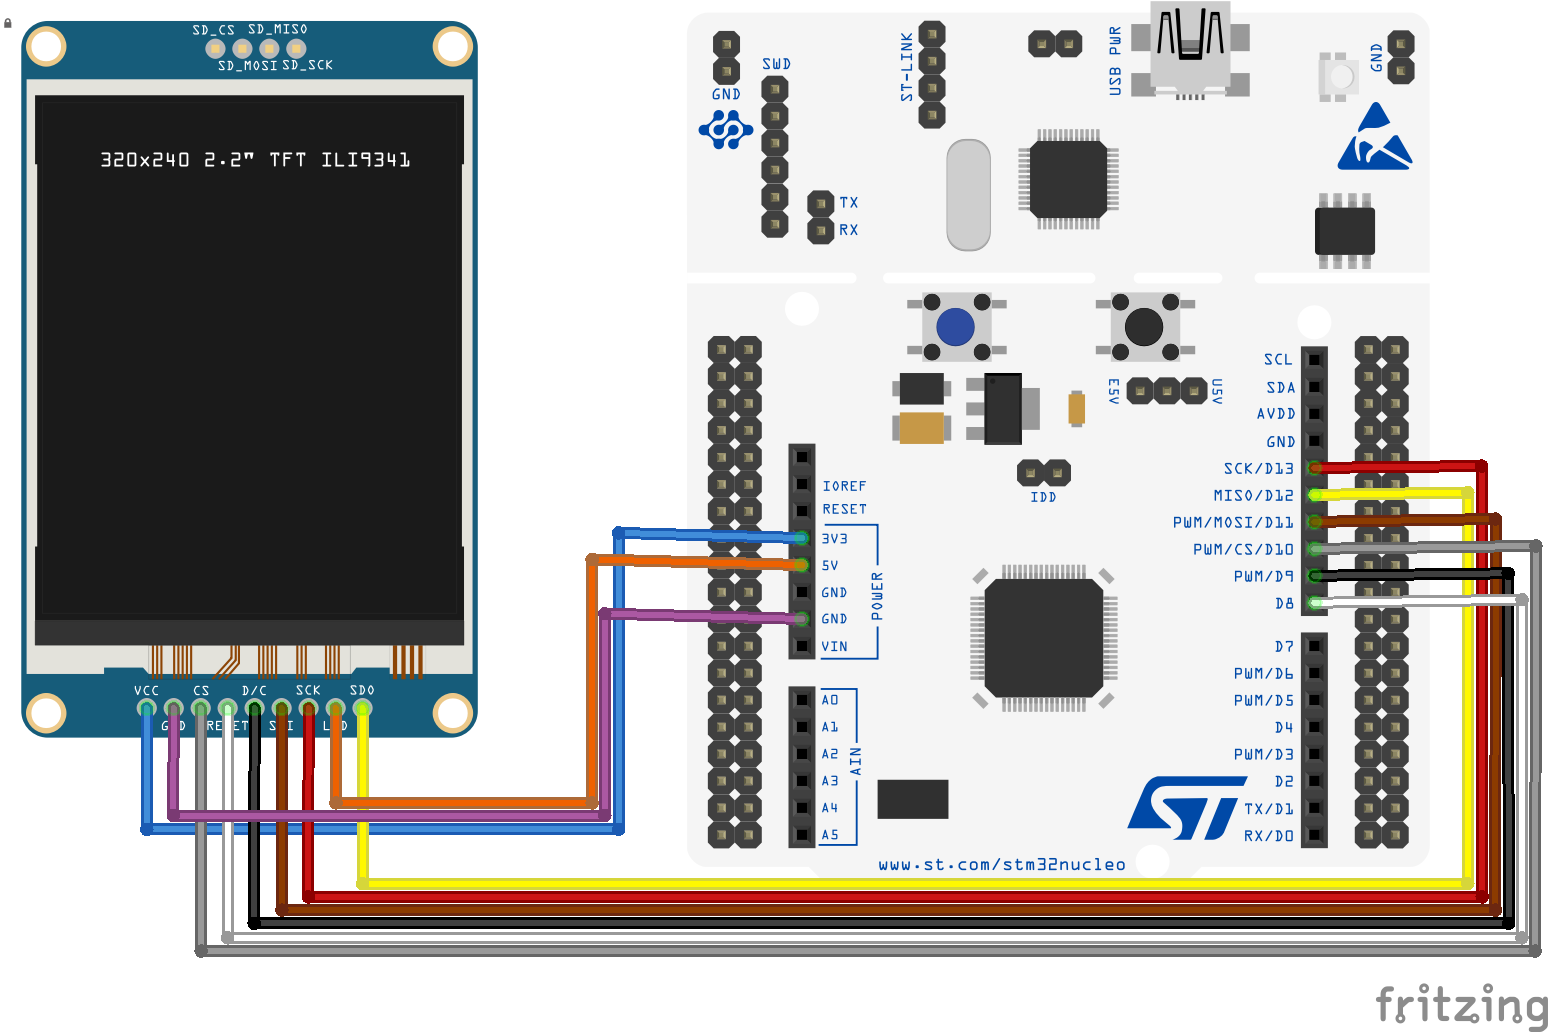
\includegraphics[width=.65\textwidth]{circuit_bb}
\end{frame}




%_____________________________________________________________
\begin{frame}{}
\begin{columns}

\column{.75\textwidth}
\begin{itemize}

\item The DHT22 digital sensor is a widely diffused component

\begin{itemize}

\item Measures temperature and relative humidity

\item Uses a custom protocol which use a single wire/bus for communication. 

\end{itemize}

\item<2> The DATA wire used for communication between STM32 MCU and the DHT22.

\begin{itemize}

\item A $4.7 K\Omega$ or $10 K\Omega$ pull-up resistor is used to bring the bus in an IDLE state when there is no communication taking place.

\item A continuous HIGH on the line denote an IDLE state.

\item The STM32 MCU acts as the bus controller and hence is responsible for initiating communication (i.e., read).

\end{itemize}

\end{itemize}

\column{.25\textwidth}
\centering
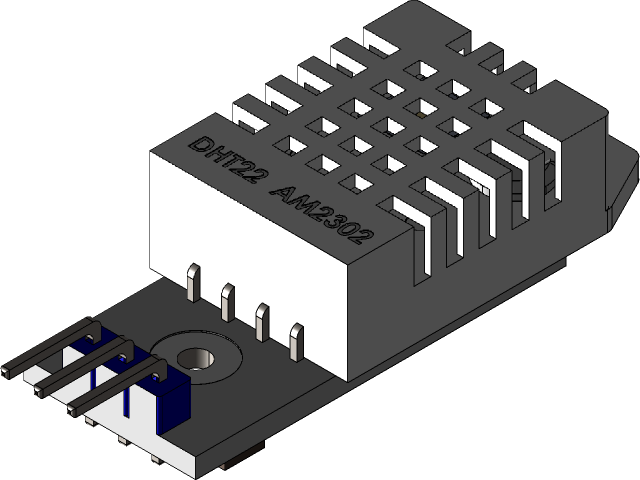
\includegraphics[width=\textwidth]{dht22}
\vspace{1cm}

\end{columns}
\end{frame}


%_____________________________________________________________
\begin{frame}{DHT22 Communication Protocol}
\begin{enumerate}

\item<1-> The STM32 MCU pulls it to a LOW for 18ms and HIGH for around $20 \ldots 40\mu s$.
\item<2-> DHT22 detects a START and responds by pulling the line LOW for $80\mu$s.
\item<3-> DHT22 pulls it HIGH for $80\mu$s which indicates that it is ready to send $40$ bits  data.
\item<4-> A bit starts with a $50 \mu$s LOW followed by $26-28\mu$s for a ``0'' or $70\mu$s for a ``1''.
\item<5> To ends, the Line is pulled HIGH by the pull-up resistor and enters IDLE state.

\end{enumerate}

\centering
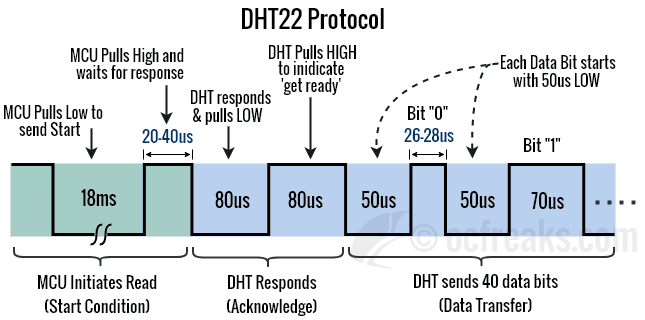
\includegraphics[width=.65\textwidth]{dht22_protocol}
\end{frame}


%_____________________________________________________________
\begin{frame}{DHT22 Data Format}
\begin{enumerate}

\item<1-> 1st Byte: Relative Humidity Integral Data in \% (Integer Part)
\item<2-> 2nd Byte: Relative Humidity Decimal Data in \% (Fractional Part) – Zero for DHT11
\item<3-> 3rd Byte: Temperature Integral in Degree Celsius (Integer Part)
\item<4-> 4th Byte: Temperature in Decimal Data in \% (Fractional Part) – Zero for DHT11
\item<5-> 5th Byte: Checksum (Last 8 bits of {1st Byte + 2nd Byte + 3rd Byte+ 4th Byte})

\end{enumerate}

\centering
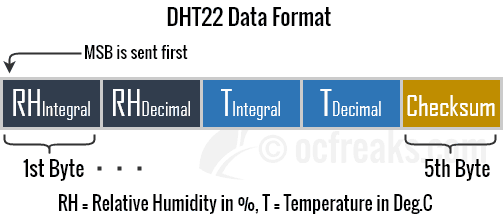
\includegraphics[width=.65\textwidth]{dht22_data_format}
\end{frame}






%=============================================================
\subsection{The RIOT operating system}
\logo{\pgfuseimage{logoRIOT}}


%_____________________________________________________________
\begin{frame}[fragile]{Creating a new application in RIOT OS -- Step 1} 
\begin{columns}

\column{.5\textwidth}
\begin{enumerate}

\item<1-> Identify location of RIOT folder\\e.g., \alert{\mintinline{bash}{/home/ichatz/RIOT}}

\item<2-> Create a new folder\\e.g., \alert{\mintinline{bash}{/home/ichatz/myapp}}

\item<3-> Create a file named \mintinline{bash}{Makefile} using your favorite editor.

\item<4-> Insert the contents provided here.

\item<5-> Change QUIET from 0 $\rightarrow$ 1 to see the compiler invocation commands. 

\item<6-> Change DEVELHELP from 1 $\rightarrow$ 0 to remove debug information.

\seti

\end{enumerate}

\column{.55\textwidth}
\vspace{-.5cm}
\begin{exampleblock}{Makefile}
\begin{minted}{c}
APPLICATION = myapp

BOARD ?= nucleo-f401re

RIOTBASE ?= $(CURDIR)/../RIOT

DEVELHELP ?= 1
QUIET ?= 0

include $(RIOTBASE)/Makefile.include
\end{minted}
\end{exampleblock}
%$

\end{columns}
\vspace{5cm}
\end{frame}


%_____________________________________________________________
\begin{frame}[fragile]{Creating a new application in RIOT OS -- Step 2} 

\begin{enumerate}

\conti

\item<1-> Create the file named \mintinline{bash}{main.c} file using your favorite editor.

\item<2-> Insert the contents provided here.

\seti

\end{enumerate}

\vspace{.5cm}

\begin{exampleblock}{main.c}
\begin{minted}{c}
#include <stdio.h>

int main(void) {
    printf("RIOT empty app.\n");
    return 0;
}
\end{minted}
\end{exampleblock}
%$

\vspace{4cm}
\end{frame}


%_____________________________________________________________
\begin{frame}[fragile]{Creating a new application in RIOT OS -- Step 3} 

\begin{enumerate}

\conti

\item<1-> Open a terminal and go to the folder of the RIOT application\\
e.g., \alert{\mintinline{bash}{/home/ichatz/myapp}}

\item<2-> Compile the code using \mintinline{bash}{make}

\item<3-> Program the STM32 board using \mintinline{bash}{make flash}

\item<4-> Connect to the STM32 board through the USB to check debug output
using \mintinline{bash}{make term}

\end{enumerate}

\vspace{.2cm}

\begin{columns}

\column{.7\textwidth}
\begin{alertblock}{Command line}
\begin{minted}{bash}
ichatz:~/# cd myapp
ichatz:~/myapp# make
ichatz:~/myapp# make flash
ichatz:~/myapp# make term
\end{minted}
\end{alertblock}
%$

\column{.2\textwidth}

\end{columns}

\vspace{4cm}
\end{frame}


%_____________________________________________________________
\begin{frame}[fragile]{Hardware Independent elements}
\vspace{-.5cm}
\begin{columns}

\column{.52\textwidth}
\begin{exampleblock}{Makefile}
\begin{minted}{c}
APPLICATION = myapp
BOARD ?= nucleo-f401re
RIOTBASE ?= $(CURDIR)/../RIOT

# Modules to include:
USEMODULE += dht
USEMODULE += fmt	

DEVELHELP ?= 1
QUIET ?= 0
include $(RIOTBASE)/Makefile.include
\end{minted}
\end{exampleblock}
%$

\column{.45\textwidth}

\vspace{1.45cm}

$\leftarrow$ We wish to use the \alert{DHT module}.\\
$\leftarrow$ \alert{FMT} = Format Module to help with the DHT protocol.

\end{columns}
\vspace{.5cm}
\end{frame}



%_____________________________________________________________
\begin{frame}{}
\vspace{.2cm}
\hspace*{1cm}
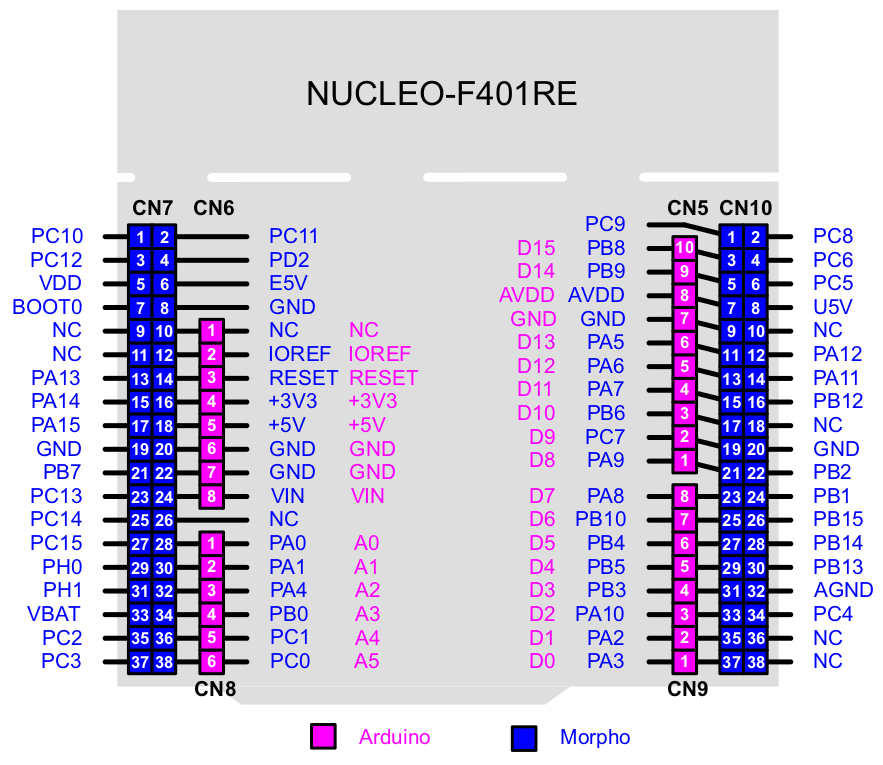
\includegraphics[width=.63\textwidth]{pinouts}
\end{frame}


%_____________________________________________________________
\begin{frame}[fragile]{}

\begin{exampleblock}{main.c}
\begin{minted}{c}
int main(void) {
    dht_params_t my_params;
    my_params.pin = GPIO_PIN(PORT_A, 10);
    my_params.type = DHT_PARAM_TYPE;
    my_params.in_mode = DHT_PARAM_PULL;

    dht_t dev;
    if (dht_init(&dev, &my_params) == DHT_OK) {
        printf("DHT sensor connected\n");
    }
}
\end{minted}
\end{exampleblock}

\begin{itemize}

\item Use the \mintinline{c}{struct dht_params_t} to provide the PIN used.

\end{itemize}

\vspace{5cm}
\end{frame}





%_____________________________________________________________
\begin{frame}[fragile]{}

\begin{exampleblock}{}
\begin{minted}[fontsize=\small]{c}
int main(void) {
    int16_t temp, hum;
    if (dht_read(&dev, &temp, &hum) != DHT_OK) {
        printf("Error reading values\n");
    }
    
    char temp_s[10];
    size_t n = fmt_s16_dfp(temp_s, temp, -1);
    temp_s[n] = '\0';
    
    char hum_s[10];
    n = fmt_s16_dfp(hum_s, hum, -1);
    hum_s[n] = '\0';        

    printf("DHT values - temp: %s°C - relative humidity: %s%%\n",
           temp_s, hum_s);
}
\end{minted}
\end{exampleblock}
\vspace{2cm}
\end{frame}


%_____________________________________________________________
\begin{frame}[fragile]{}

\begin{alertblock}{Command line}
\begin{minted}{bash}
ichatz:~/# cd myapp
ichatz:~/myapp# make flash 
ichatz:~/myapp# make term
/home/ichatz/RIOT/dist/tools/pyterm/pyterm -p "/dev/ttyACM0" -b "115200"  
Twisted not available, please install it if you want to use pyterm's JSON capabilities
# Connect to serial port /dev/ttyACM0
Welcome to pyterm!
Type '/exit' to exit.
# DHT sensor connected
# DHT values - temp: 21.8°C - relative humidity: 46.9%
\end{minted}
\end{alertblock}
%$
\vspace{2cm}
\end{frame}

\end{document}

